\documentclass{article}

% if you need to pass options to natbib, use, e.g.:
% \PassOptionsToPackage{numbers, compress}{natbib}
% before loading nips_2018

% ready for submission
\usepackage{nips_2018}
\usepackage{graphicx}

% to compile a preprint version, e.g., for submission to arXiv, add
% add the [preprint] option:
% \usepackage[preprint]{nips_2018}

% to compile a camera-ready version, add the [final] option, e.g.:
% \usepackage[final]{nips_2018}

% to avoid loading the natbib package, add option nonatbib:
% \usepackage[nonatbib]{nips_2018}

\usepackage[utf8]{inputenc} % allow utf-8 input
\usepackage[T1]{fontenc}    % use 8-bit T1 fonts
\usepackage{hyperref}       % hyperlinks
\usepackage{url}            % simple URL typesetting
\usepackage{booktabs}       % professional-quahttps://www.overleaf.com/project/5bbd5cc96115aa7a36833fc9lity tables
\usepackage{amsfonts}       % blackboard math symbols
\usepackage{nicefrac}       % compact symbols for 1/2, etc.
\usepackage{microtype}      % microtypography

\title{Final Report}

\author{
   Malik Majette \\
  North Carolina State University\\
%   Address \\
   \texttt{mamajett@ncsu.edu} \\
   \And
   Qua Jones \\
  North Carolina State University\\
%   Address \\
   \texttt{qyjones@ncsu.edu} \\
   \AND
   Wenting Zheng\\
  North Carolina State University\\
%   Address \\
   \texttt{wzheng8@ncsu.edu} \\
}

\begin{document}
% \nipsfinalcopy is no longer used
\maketitle


\section{Background}
Each year the National Basketball Association (NBA), media, and fans of the sport vote to select the season’s 24 All-Stars. 5 players from the Eastern and Western conference are chosen based on the highest number of votes, with fan votes weighing 50\%, media votes weighing 25\%, and NBA player votes weighing the remaining 25\%. These 10 players will represent the starting line-up in the All-Star game for their respective conferences. The remaining 14 players are picked by NBA head coaches based on statistics and player abilities. Although some players, like LeBron James, are chosen year-to-year, for many NBA players there is an amount of uncertainty on whether or not they will be picked. We hypothesize that by using NBA statistics from previous years we can develop a classification-based determination of future All-Stars.

\section{Method}

The classification-based approach incorporates a decision tree, k-Nearest Neighbors, and Neural Network to determine the 2017-2018 All-Stars. Each model uses All-Star player data from 2014-2017 to a construct a classification for all 2017-2018 players. The misclassification rate for each model is compared to determine the best classifier for this problem. All models will be built on the same attributes (listed in Table 1) and supervised anomaly detection is implemented as well to determine which attributes weigh heaviest in correctly classifying an All-Star. Based on our results data scientists will have more information on the strongest classifier for this domain and NBA players will have a better understanding of if they will become an All-Star and which statistic lines impacted their chances the most.
See
Table~\ref{attribute-table}.

\begin{table}
  \caption{Attribute Table}
  \label{attribute-table}
  \centering
  \begin{tabular}{llll}
    \toprule
    Attribute & Description & Attribute & Description \\
    \midrule
    AGE     & Age   & 3P\% &  Three-Pointer Percentage \\
    GP &  Games Played & FTM & Free-Throws Made\\
    W& Win &  FTA & Free-Throws Attempted\\
    L & Loss & FT\% & Free-Throw Percentage\\
    MIN & Minutes Played & OREB & Offensive Rebounds\\
    PTS & Points per Game & DREB & Defensive Rebounds\\
    FGM & Field Goals Made & REB & Rebounds per Game\\
    FGA & Field Goals Attempted & AST & Assists per Game\\
    FG\% & Field Goal Percentage & TOV & Turnovers per Game\\
    3PM & Three-Pointers Made & STL & Steals per Game\\
    3PA & Three-Pointers Attempted & BLK & Blocks per Game\\
    \bottomrule
  \end{tabular}
\end{table}

\subsection{Artificial Neural Network}
The Artificial Neural Network (ANN) model is an assembly of inter-connected nodes and weighted links inspired by the biological neural networks of the animal brain. The input layer, which consists of a variable number of input nodes, is linked to a hidden layer based on a weight. Each node in the hidden layers applies an activation function to the summation of these inputs that determines a normalized output value to be passed to the next layer. When the algorithm reaches the output layer, the output node is compared to a threshold to classify the result. In supervised ANN training, the network is providing matching inputs and outputs with the intention of the network eventually producing the desired output by adjusting the weights of the connections over time. This technique will be applied to the NBA All-Star data to create a model that can classify NBA All-Stars by using data from previous year All-Stars as a training set.


\subsection{Decision Tree}
Decision Trees are a nonparametric supervised learning method for classification and regression. It builds classification models in the form of a tree structure. It breaks down a data set into smaller subsets while simultaneously incrementally developing an associated decision tree. Cross validation is a technique for evaluating models by training models on subsets of data and evaluating on the complementary of the same subset. With k-fold cross validation, data is split into k subsets and the model is trained on k-1 subsets. The model is evaluated on the subset that was not used for training, this process is repeated k times. 
  
\subsection{K-Nearest Neighbors}
K-nearest neighbors algorithm(KNN) is a nonparametric method used for classification. It is preferred if the input is continuous. The input consists of training dataset in multidimensional feature space. A defined constant(K) number of the nearest neighbors are selected based on the unknown testing input. Classification is obtained by the majority vote of the K nearest points. Generally, larger K reduces the influence of outliers and noise but also increase the risk of underfitting.

The misclassification rate depends on the training data, the K value, the distance type, and if the distance is weighted. We will use 2014-2017 NBA statistics as training data, and use Manhattan and Euclidean distance to measure the distance. Our goal is to find the best combination that minimizes the misclassification rate. 

\section{Experiment}
\subsection{Artificial Neural Network}
Our goal with ANN is to construct the best model for predicting 2017-2018 All Stars based on the training dataset, number of hidden nodes, step activation function, and output activation function. In order to construct a training dataset, the NBA statistics from 2014-2017 are loaded and concatenated into a multi-dimensional array with each column representing an attribute from the attribute table and each row representing a player. The expected output training dataset is represented as [0, 1] for non-All-Stars and All-Stars respectively. The testing dataset is the All-Star player data from 2017-2018. During the pre-processing step we apply normalization to obtain normalized training and testing datasets. Since the testing dataset is treated as unknown data, the maximum and minimum of the corresponding training dataset are used to normalize the testing dataset. This step rescales the range of the attributes in the range of [0, 1] and allows comparison between attributes and between datasets. 

Next we use these two datasets to train a neural network model with different number of hidden neurons, step activation functions, and output activation functions. Based on Jeff Heaton’s research in “Introduction to Neural Networks in Java”, the number of neurons in the hidden layer is usually the mean of the neurons in the input and output layers. With 22 input nodes and a single output node a decent number of neurons would be around 12 so the model is tested with samples over all even numbers within the space [2,24]. We choose tanh as the initial step activation function and sigmoid as the initial output activation function since they are commonly used in ANN. Both activation functions are tuned with a set of standard functions: [sigmoid, hard\_sigmoid, tanh, elu, relu]. Each trained model is evaluated against the testing dataset and compared to the actual results to compute the classification rate.


\begin{figure}
  \centering
  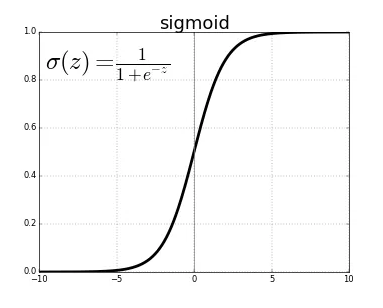
\includegraphics[width=5.5cm]{ann2.png}
  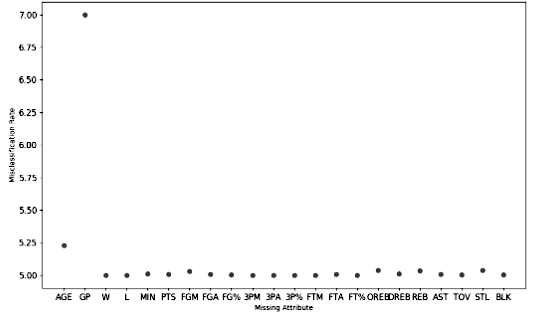
\includegraphics[width=8cm]{ann3.png}
  \caption{[left]Sigmoid Function and [right]NN Classification Dependency on Attributes}
\end{figure}

\subsection{Decision Tree}
\begin{figure}
  \centering
  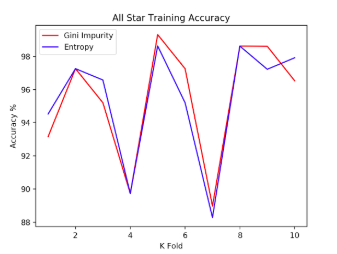
\includegraphics[width=8cm]{decisiontree.png}
  \caption{Decision Tree Accuracy}
\end{figure}

In order to construct the appropriate training set, statistics from seasons 2014-2017 were combined into a larger set of data to be processed. For classifying All-Stars [0,1] is used to represent non-All-Stars and All-Stars respectively. Two decision tree classifiers were constructed, one based on a Gini Impurity classification and one based on a Entropy classification. 10 fold cross validation was applied to the 2014-2017 dataset for model evaluation. Data from the 2017-2018 season were used for testing and to determine the accuracy of the models. The mean accuracy for the classification models were 96.67\% for Gini Impurity and 97.22\% for Entropy.


\subsection{K-Nearest Neighbors}
Our goal is to find the best combination of the training dataset, distance metric, distance weight, and K value of the KNN classifier to minimize the misclassification rate. We have All-Star player data from 2014-2017. First, data is grouped by year and there will be three training datasets. Another dataset consists of all three-year player data, so we have four training datasets in total. The testing dataset is the All-Star player data from 2017-2018. Then, we apply normalization to obtain normalized training and testing datasets in the pre-processing stage. Since the testing dataset is treated as unknown data, the maximum and minimum of the corresponding training dataset are used to normalize the testing dataset. This step rescales the range of the attributes in the range of [0, 1] and allows comparison between attributes and between datasets. 

Next, we use these four datasets to individually train the KNN classifier with different distance metrics, weight, and the K values. We choose Euclidean and Manhattan distance metrics since they are widely used in KNN. All the neighbors will be assigned with uniform weight or weight that is inversely dependent on distance. That is to say, closer neighbors will have greater weight and influence than the further neighbors. Since the uniform weight method is more sensitive to the neighbors that are on the edge, we expect the weighted classifiers will have better performance than the uniform one. Choose a reasonable range of k reduces time to compute the misclassification rate. We first run the program with two datasets and discovered the misclassification rate line is a horizontal line when k is around 50. In this case, we choose the k values to be the integers in the range of [1, 50]. 

The trained classifier is applied to the testing dataset in order to predict if the player would be an All-Star player. Then predicted results are compared to the actual results to compute the error rate. If the predicted values are continuous instead of discrete, we should have an extra step of categorization. For example, if the predicted values are in the range of [0, 1]. We need to assign [0, 0.5] to be ‘No’ class. Since the predicted values are binary, we are able to directly calculate the error rate by misclassified objects/total number of objects.


\section{Result}
\subsection{Artificial Neural Network}
\begin{figure}
  \centering
  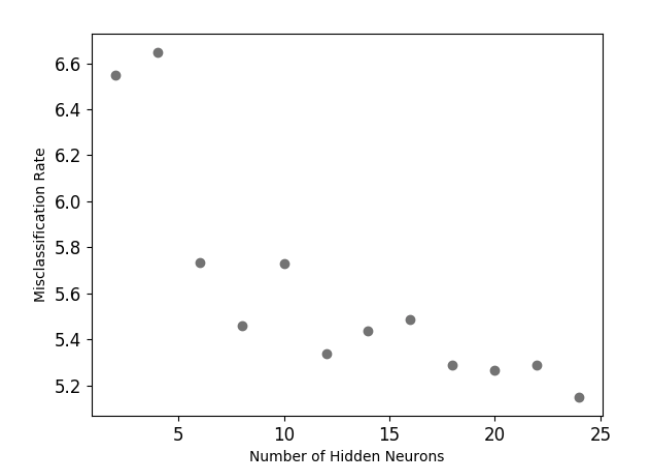
\includegraphics[width=6.3cm]{ann_hidden.png}
  \caption{Error rate based on number of hidden neurons}
  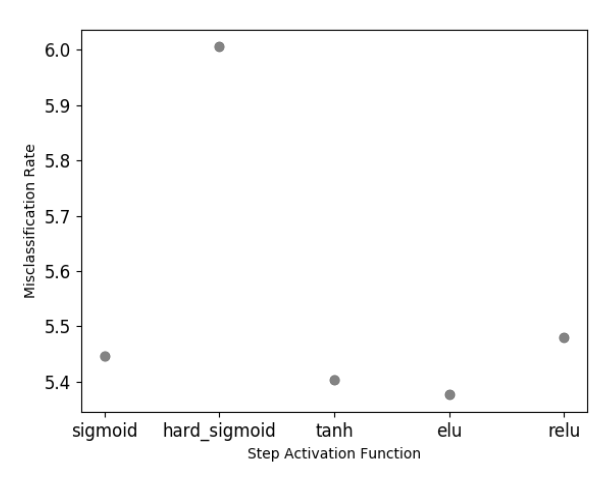
\includegraphics[width=5.5cm]{ann_step.png}
  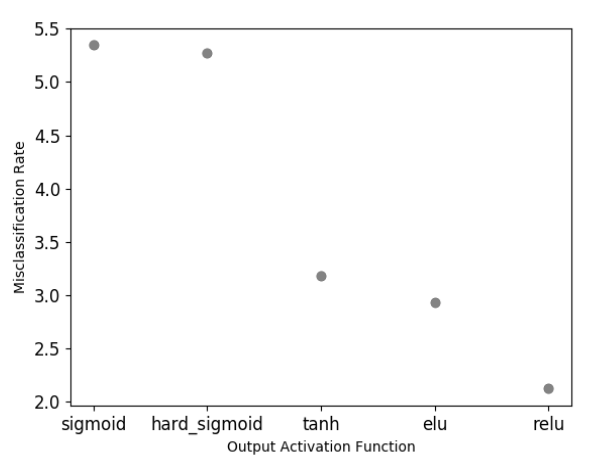
\includegraphics[width=6cm]{ann_output.png}
  \caption{[left] Error rate based on step activation and output activation function [right]}
\end{figure}
The following plots represent the misclassification rate based on the number of hidden neurons, step activation function, and output activation function. The number of hidden neurons was the first tuned parameter. Over [2, 24] with tanh as the initial step activation function and sigmoid as the initial output activation function, the optimal number of hidden neurons is 24. We notice that as the number of neurons increase the misclassification rate gradually decreases. However, continuing to use values higher than 24 would increase the complexity of the model and lead to overfitting. Using this result and keeping the output activation function as sigmoid, the step activation is then tuned based on the set of standard functions. All functions resulted in relatively equal misclassification rates except hard\_sigmoid. The step activation function with the minimum misclassification rate was ELU (Exponential Linear Unit). Since ELU zeroes out less relevant signals the function is optimal for datasets with attributes of varying significance to the result. Finally, with the results of the previous two tuned parameters the output activation function is determined. Again the function is tuned based on the set of standard functions and ReLU (Rectified Linear Unit) is the resulting optimal output function. We find that the minimal misclassification rate based on the optimal number of hidden neurons, step activation function, and output activation function is 2.054\%.

\subsection{Decision Tree}
The following plot represents the misclassification rate based on the K value, and the type of classifier. The k value was the first tuned parameter, initially I chose a k value of 10 as a good starting place. To get a clearer picture of how the K value was affecting the misclassification rate, we decided to expand the range to [2,10]. When tweaking the k value, we also decided to see if using a random splitter revealed a better performance than the ‘best’ splitter. This proved to no avail with a visible overall increase in misclassification rates. In the figure below we can see the misclassification rate for k values ranging from 2 - 10. Based on the graph, entropy seems to have a lower misclassification rate compared to Gini Impurity with the lowest rate being seen with k = 2 for an error rate lower that 3.2\%. For Gini Impurity, the lowest error rate can also be seen with the k = 2 value however the error rate for this classification is closer to 3.4\%. With an increase in k value we see an overall increase in error rate, with gini impurity often having the higher misclassification rate than the entropy classifier. For both the Gini and Entropy decision trees, the first split was PTS which is the number of points per game of a player. This is the most important feature in appropriately classifying an ALL-STAR.

\begin{figure}
  \centering
  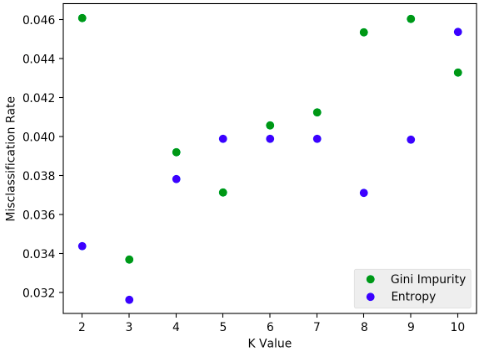
\includegraphics[width=6.8cm]{decision_training_error.png}
  \caption{All Star Training Misclassification}
\end{figure}

The classification reports of the decision tree classifiers reveals that both classifiers have comparable rates when non ALL Star players are classified with Entropy having a slightly higher precision rate (1\% higher). Gini exhibits a less efficient ability of classifying All Star players with rates of .67, .81, and .73 for precision, recall, and f1-score respectively.  Entropy consistently outperforms the Gini Impurity classifier with an average error rate of 2.9\%.


\begin{figure}
  \centering
  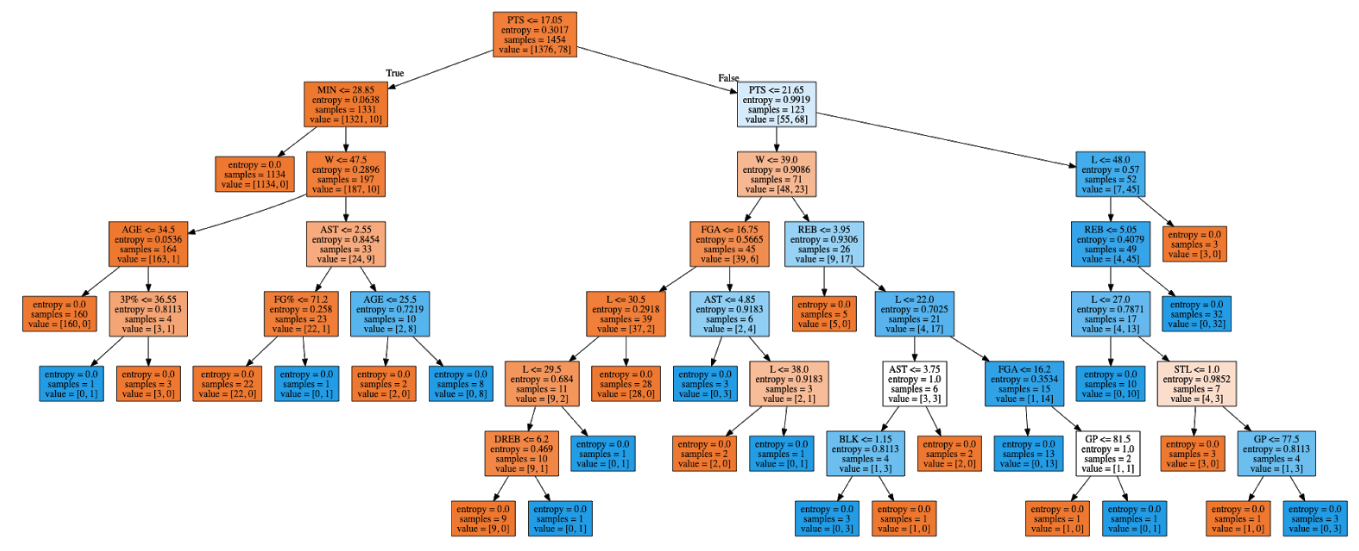
\includegraphics[width=10cm]{gini_decission.png}
  \caption{Gini Decision Tree}
\end{figure}

\begin{figure}
  \centering
  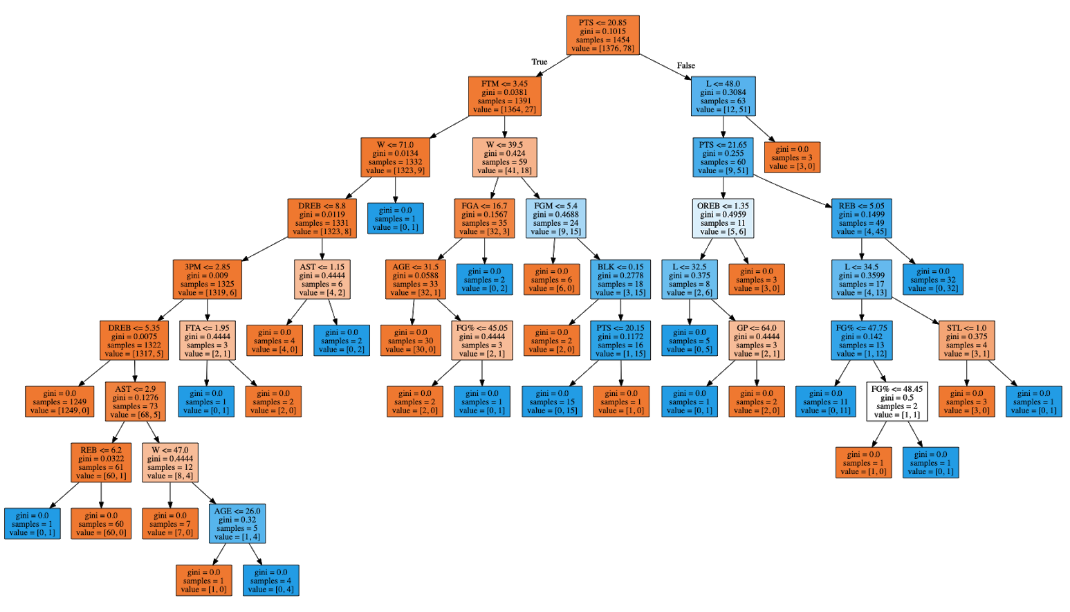
\includegraphics[width=10cm]{entropy_decision.png}
  \caption{Entropy Decision Tree}
\end{figure}

\begin{table}
  \caption{Gini Decision Tree Classification Reports}
  Error Rate: 0.035
  \label{DT_Gini}
  \centering
  
  \begin{tabular}{lllll}
    \toprule
     & Precision & Recall & FL-score & Support\\
    \midrule
    0 & .98 & .98 & .98 & 513 \\
    1 & .63 & .70 & .67 & 27 \\
    avg/total & .97 & .96 & .97 & 540 \\
    \bottomrule
  \end{tabular}
\end{table}

\begin{table}
  \caption{Entropy Decision Tree Classification Reports}
  Error Rate: 0.029
  \label{DT_Entropy}
  \centering
  
  \begin{tabular}{lllll}
    \toprule
     & Precision & Recall & FL-score & Support\\
    \midrule
    0 & .99 & .98 & .98 & 513 \\
    1 & .67 & .81 & .73 & 27 \\
    avg/total & .97 & .97 & .97 & 540 \\
    \bottomrule
  \end{tabular}
\end{table}

\subsection{k-Nearest Neighbors}
The following plots represent the misclassification rate based on the K value and distance weight. Since we have four training datasets, there are four graphs for Euclidean and Manhattan distance. Each graph contains two lines. The dashed line is the error rate with weighted distance while the solid line is with uniform weigh. The weighted distance emphasizes the importance of the closer neighbors in the multidimensional feature space, which may indicate the higher similarity between neighbors and predicted point. Therefore, we expected weighted line has higher accuracy and lower error rate in the graph. From the graph, it’s obvious that the weighted distance generally performs better since the dashed lines are mostly below the solid line in all the graphs, which confirms our expectation. 

Additionally, a clear trend is found in each session’s figure. The error rate is initially around 3\%-3.5\% and drops gradually with the increase of k value. The best range of the k value is around [5, 15] where the minimal misclassification rate occurs the most. Then, the error rate steadily climbs as k value increases and reaches the maximal error rate when k is around 45. The relatively high error rate when k is small is because of overfitting. That is to say, the classifier fits the neighbor too much when k value is small. For example, very small K may accidentally select noisy points from the dataset, which results in the lower accuracy. On the other hand, underfitting causes the increase of the error rate when k value is too large. Including more data from the other categories results in more misclassified points. 

\begin{figure}
  \centering
  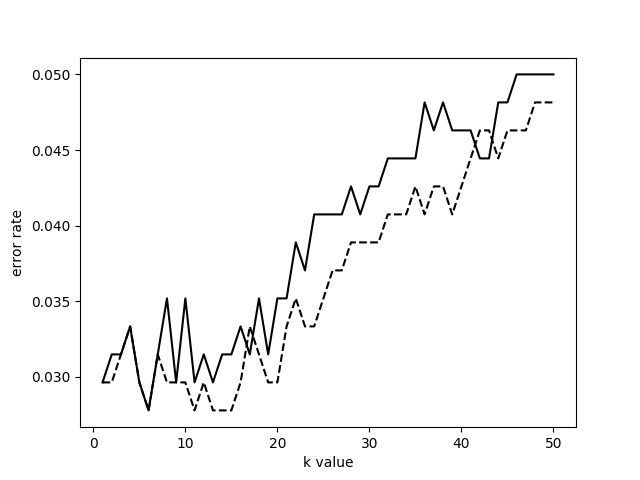
\includegraphics[width=6.3cm]{knn_err14.png}
  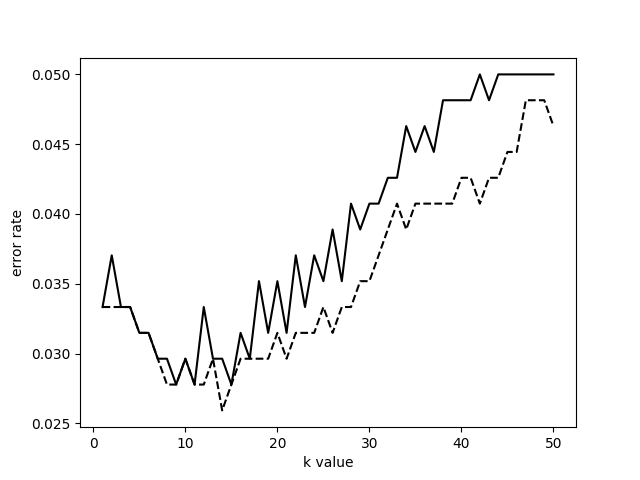
\includegraphics[width=6.3cm]{knn_err15.png}
  \caption{(Euclidean)Error rate with 2014-2015[left top] and 2015-2016[right top]
  }
  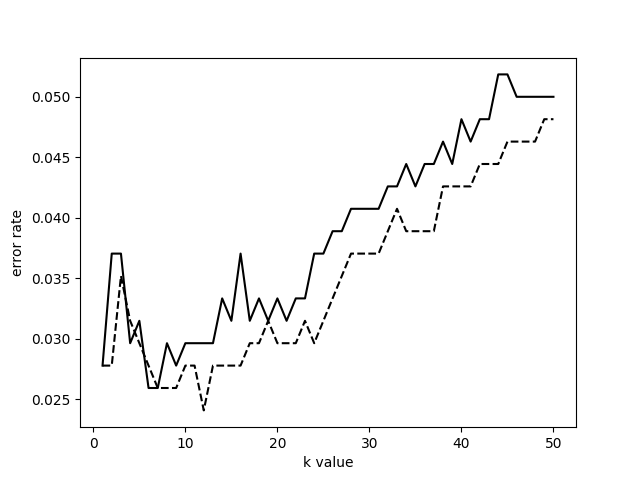
\includegraphics[width=6.3cm]{knn_err16.png}
  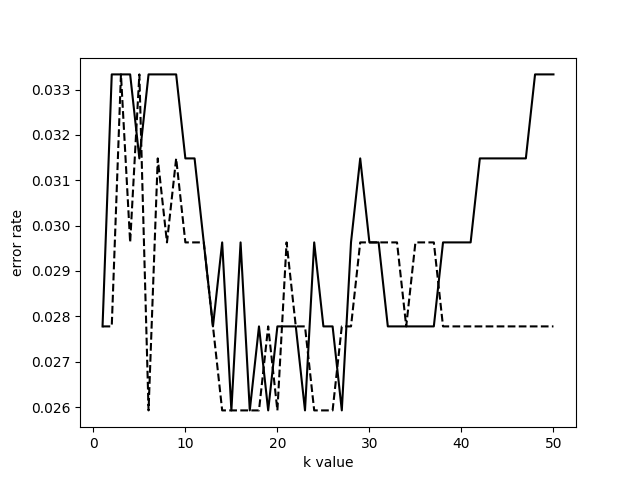
\includegraphics[width=6.3cm]{knn_errall.png}
  \caption{(Euclidean)Error rate with 2016-2017[left bottom] and 2014-2017[right bottom]}
\end{figure}


However, the error rate of the three-year dataset is comparatively fluctuant and doesn’t show this trend. One observation is that more neighbor points are needed when we use 2014-2017 dataset and uniform weight. It’s probably because the data from other years in considered as noise and more data in needed to make a relatively accurate prediction. The other observation is its accuracy. We expected a higher accuracy in three-year dataset due to its larger size. However, no evidence found in Table~\ref{Min-MR-table} shows a lower error rate in 2014-2017 column, which is surprising.

By looking at the minimal misclassification rate in each graph, Manhattan metric has slightly lower misclassification rate but there is no much difference between Euclidean and Manhattan distance functions. When we use the Euclidean distance, the minimal error rate is 2.41\% when classifier is trained by 2016-2017 dataset and k is 12. When we use Manhattan distance, the minimal error rate doesn’t change but it occurs in several conditions. 2.41\% occurs when we use 2015-2016 player data as training dataset and set k value as 10(weighted) or 11(uniform). It also occurs when three-year data is used to train classifier with k = 24. We will select the minimal k value in this case since it’s the simpler model. Therefore, the best combination to minimize the misclassification error rate is using 2015-2016 training dataset in KNN with weighted Manhattan distance when value of k is 10. 

\begin{figure}
  \centering
  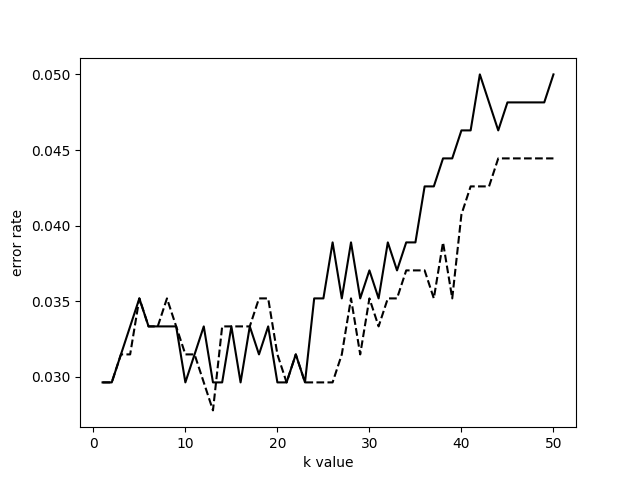
\includegraphics[width=6.3cm]{knn_err14_ma.png}
  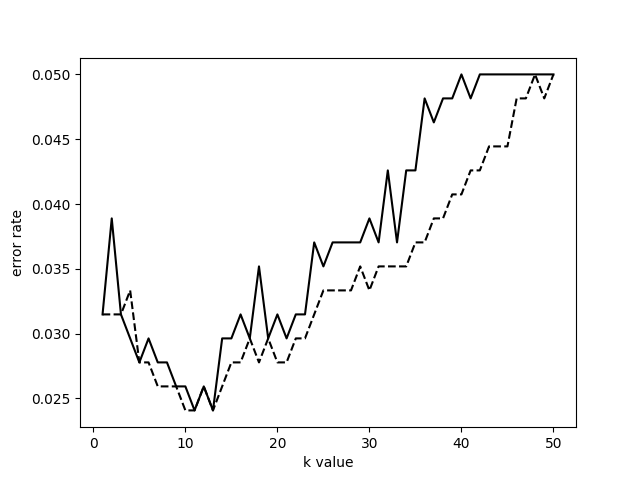
\includegraphics[width=6.3cm]{knn_err15_ma.png}
  \caption{(Manhattan)Error rate with 2014-2015[left top] and 2015-2016[right top]}
  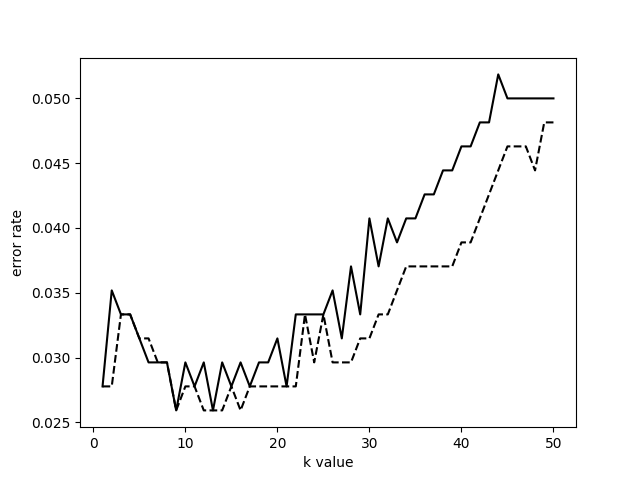
\includegraphics[width=6.3cm]{knn_err16_ma.png}
  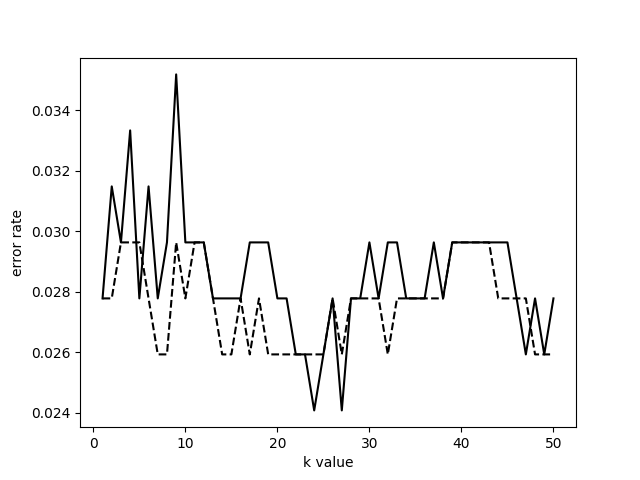
\includegraphics[width=6.3cm]{knn_errall_ma.png}
  \caption{(Manhattan)Error rate with 2016-2017[left bottom] and 2014-2017[right bottom]}
\end{figure}

\begin{table}
  \caption{Minimal Misclassification Rate Table}
  \label{Min-MR-table}
  \centering
  \begin{tabular}{llllll}
    \toprule
    Distance Metric & Weight & 2014-2015 & 2015-2016 & 2016-2017 & 2014-2017\\
    \midrule
    Euclidean & Uniform     & 0.0278, k=6   & 0.0278, k=9 & 0.0259, k=6 & 0.0259, k=15\\
    Euclidean & Weighted &  0.0278, k=6   & 0.0259, k=14 & 0.0241, k=12 & 0.0259, k=6\\
    Manhattan & Uniform     & 0.0296, k=1   & 0.0241, k=11 & 0.0259, k=9 & 0.0241, k=24\\
    Manhattan & Weighted &  0.0278, k=13   & 0.0241, k=10 & 0.0259, k=9 & 0.0259, k=7\\
    \bottomrule
  \end{tabular}
\end{table}


\section{Conclusion}
Using three distinctive classification methods we found that all models were able to make accurate predictions of an All-Star player based on statistics from players in previous years. Artificial Neural Network, Decision Tree, and K-Nearest Neighbors all performed with a misclassification rate lower than 3\% after tuning respective variables that affect the accuracy of classification. The minimal misclassification rate was achieved with ANN at 2.054\%. This result is fairly expected since ANN’s model of classifying data sets based on weights is the most complex and handles numerical data extremely well. Although, Decision Trees and KNN provide their own benefits to the problem by presenting a visual representation of how the model is classifying data, compared to ANN which is essentially a black box. By evaluating the top node of the Gini decision tree we see that points per game (PTS) is the strongest indicator for All-Stars and non All-Stars. This eliminates the extra steps that would have been needed in ANN in order to determine which statistic lines impacted their chances the most. Overall, all three models develop strong classification algorithms, and the methods and results used compliment each other to provide a holistic understanding of how to classify NBA All-Stars.

\section*{References}
\small
[1] Kim, Keon. (2017) Deep Q-Learning with Keras and Gym. {\it Deep Q-Learning with Keras and Gym.} keon.io/deep-q-learning/.

[2] Staff, NBA.com (2018) How the NBA All-Star Draft Works. {\it How the NBA All-Star Draft Works. } www.nba.com/article/2018/01/18/2018-nba-all-star-draft-rules.

\end{document}
